\documentclass[9pt,technote]{IEEEtran}
%\documentclass{article}

\usepackage[numbers,sort&compress]{natbib}
\usepackage{natbib}
\usepackage{url}
\usepackage[]{hyperref}
\usepackage{cleveref}
\usepackage{verbatim}
\usepackage{amsmath,amssymb}
\usepackage{rotating}
\usepackage{tikz}

\author{Aaron McDaid, Derek Greene, Neil Hurley}
\title{Mutual Information for overlapping groupings}
\begin{document}

\maketitle


\newcommand{\grouping}{\emph{grouping{}}}
\newcommand{\lfk}{\cite{lancichinetti-2009} {}}

\begin{abstract}
Given the increasing popularity of algorithms for overlapping clustering, in particular in social network analysis, quantitative measures are needed to measure the accuracy of a method.
Given a set of true clusters, and the set of clusters found by an algorithm, these sets of sets must be compared to see how similar or different the sets are.
A normalized measure is desirable in many contexts, for example assigning a value of 0 where the two sets are totally dissimilar, and 1 where they are identical.

A measure based on normalized mutual information has recently become popular. We demonstrate unintuitive behaviour of this measure, and show how this can be corrected
by using a more conventional normalization. We compare the results to that of other measures, such as the Omega index \cite{collins1988omega}.
\end{abstract}


In a non-overlapping scenario, each node belongs to exactly one cluster. We are looking at overlapping, where a node could belong to many communities, or indeed to no clusters.
Such a set of clusters has been referred to as a \emph{cover} in the literature, and this is the terminology that we will use.

For a good introduction to our problem of comparing covers of overlapping clusters, see \cite{collins1988omega}.
They describe the Rand index, which is defined only for disjoint clusters, and then show how to extend it to overlapping clusters.
Each pair of nodes is considered and the number of clusters in common between the pair is counted. Even if a typical node is in many clusters,
it's likely that a randomly chosen pair of nodes will have zero clusters in common.
%If there are $n$ objects, there are $N=\frac12 N(N-1)$
These counts are calculated for both covers and the Omega index is defined as the proportion of pairs for which the shared-cluster-count is identical,
subject to a correction for chance.

\section{Mutual information}

Meila (which paper to reference?) defined a measure based on mutual information for comparing disjoint clusterings.
\citet{lancichinetti-2009} proposed a measure also based on mutual information, extended for covers.
This measure has become quite popular for comparing community finding algorithms in social network analysis.
It is the measure we are primarily concerned with there, and we will refer to it as LFKNMI named after the authors.

We are proposing to use a different normalization, but first we will define the non-normalized measure.
For full details, look at the final section of \citet{lancichinetti-2009}.

Given two covers, $X$ and $Y$, we must first see how to measure the similarity between a pair of clusters.
$X$ and $Y$ are matrices of cluster membership. There are $n$ objects.
The first cover has $K_X$ clusters, and hence $X$ is an
$n \times K_X$ matrix. $Y$ is an $n \times K_Y$ matrix.

To compare cluster $i$ of the first cover to cluster $j$ of the second cover, we compare the vectors
$X_i$ and $Y_j$. These are vectors of ones and zeroes.

\begin{itemize}
	\item $              { a = \sum_{m=1}^n [X_{i,m} = 0 \wedge  Y_{j,m} = 0] } $
	\item $              { b = \sum_{m=1}^n [X_{i,m} = 0 \wedge  Y_{j,m} = 1] } $
	\item $              { c = \sum_{m=1}^n [X_{i,m} = 1 \wedge  Y_{j,m} = 0] } $
	\item $              { d = \sum_{m=1}^n [X_{i,m} = 1 \wedge  Y_{j,m} = 1] } $
\end{itemize}

If $a+d = n$, and therefore $b=c=0$, then the two vectors are in complete agreement.

The lack of information between two vectors is defined:
\begin{align}
	H(X_i | Y_j) = & {} H(X_i , Y_j) - H(Y_j)  \\
	               = & {} h(a,n) + h(b,n) + h(c,n) + h(d,n)  \\ 
		         & {} - h(b+d,n) - h(a+c,n)
\end{align}
where $h(w,n) = -w \log_2 \frac{w}{n} $

There is an interesting technicality here. Imagine a pair of clusters but where the memberships
have been defined randomly.
There is a possibility that there will be a small amount of mutual information, even in this situation where the two vectors are negatively correlated with each other.
In extremis, if the two vectors are near complements of each other, mutual information will be very high. We wish to override this and define that
there is zero mutual information in this case.
% The mutual information should be positive if and only if the correlation is positive (can we include this?)
This is defined in equation (B.14) of \cite{lancichinetti-2009}.
We also use this restriction in our proposal.

\begin{equation}
	\begin{split}
	H^* & (X_i | Y_j) = \\
	& \left\{
		\begin{split}
			H^*(X_i | Y_j) \; & \mbox{if} \; h(a,n) + h(d,n) \geq h(b,n) + h(c,n) \\
			h(c+d,n)+h(a+b,n) \;  & \mbox{otherwise}
		\end{split}
	\right.
	\end{split}
	\label{eqnNoComplements}
\end{equation}

This allows us to compare vectors $X_i$ and $Y_j$, but we want to compare the entire matrices
$X$ and $Y$ to each other. We will follow the approximation used by \lfk here and
match each vector in $X$ to its best match in $Y$,

\begin{equation}
	H(X_i | Y) = \underset{j \in \{1,\dots K_Y \}}{\min} H(X_i | Y_j)
	\label{eqnBestMatch}
\end{equation}

then summing across all the vectors in $X$,

\begin{equation}
	H(X | Y) = \sum_{i \in \{1,\dots K_X \}} H(X_i | Y)
	\label{eqnSumVectors}
\end{equation}

$H(Y|X)$ is defined in a similar way to $H(X|Y)$, but with the roles reversed.

\section{Useful identities}

\begin{figure}
	\centering
\begin{tikzpicture}
	\draw (-1cm,0) circle(2cm);
	\draw (1cm,0) circle(2cm);
	\draw (0,0cm) node[fill=white] {$I(X:Y)$};
	\draw (1.8cm,0cm) node[fill=white] {$H(Y|X)$};
	\draw (-1.8cm,0cm) node[fill=white] {$H(X|Y)$};
	\path(1cm,0) ++  (60:2.2cm) node[rotate=-25] {$H(Y)$};
	\path(-1cm,0) ++ (120:2.2cm) node[rotate= 25] {$H(X)$};
\end{tikzpicture}
\caption{\label{figVenn} Mutual information and variation of information. The total information $H(X,Y) = H(X|Y) + I(X:Y) + H(Y|X)$. }
\end{figure}


\cref{figVenn} gives us an easy way to remember the following useful identities, which
apply to any mutual information context.

\begin{align*}
	H(X) = & I(X:Y) + H(X|Y) \\
	H(Y) = & I(X:Y) + H(Y|X) \\
	H(X,Y) = & H(X) + H(Y|X) \\
	H(X,Y) = & H(Y) + H(X|Y) \\
	H(X,Y) = & \overbrace{I(X:Y)}^\text{mutual information} + \overbrace{H(X|Y) + H(Y|X)}^\text{variation of information}
\end{align*}

This gives us two definitions for the mutual information, $I(X:Y)$.
In theory, these should be identical, but due to the nature of \cref{eqnBestMatch}
they may be different. Therefore, we will use the average of the two.

\begin{equation}
	I(X:Y) := \frac12 \left[ H(X)-H(X|Y) + H(Y)-H(Y|X) \right]
	\label{eqnAverageOfTwo}
\end{equation}

We are now ready to discuss normalization, contrasting the method of \lfk
with our alternative.

\citet{lancichinetti-2009} define their own normalization of the \emph{variation of information},
\begin{equation}
	VI_{normalized}(X,Y) = \frac12 \left(  \frac{ H(X|Y) }{ H(X) } + \frac{ H(Y|X) }{ H(Y) } \right)   \label{VOI}
\end{equation}
and hence their normalized mutual information is
\begin{equation}
	I_{normalized}(X,Y) = 1 - \frac12 \left(  \frac{ H(X|Y) }{ H(X) } + \frac{ H(Y|X) }{ H(Y) } \right) %  \label{VOI}
\end{equation}

There are of course many ways to normalize a quantity such as the \emph{variation of information}.
Normalization typically involves division by a quantity $c$,
\begin{equation}
	\frac{ H(X|Y) + H(Y|X) } {c(X,Y)} \label{eqnNorms}
\end{equation}
where $c$ is a function of $X$ and $Y$ which is guaranteed to be less than or equal to the numerator.
But LFKNMI does not use a normalization of this standard form, instead using \cref{VOI}.

There is another aspect to the non-standard normalization used in LFKNMI;
they insert an extra normalization factor into their definition of $H(X_i|Y_j)$.
But this is not the root cause of the problems we will describe, hence we will not dwell on it.
Our change is to remove all the normalization steps from their analysis and instead
use a more conventional normalization of the form of \cref{eqnNorms}.

\section{Unintuitive behaviour of LFKNMI}
\label{secUnintuitive}
There are circumstances where LFKNMI overestimates the similarity of two clusters.
We will show how an alternative normalization will fix these problems.

Imagine a cover $X$, and we are comparing it to a cover $Y$. Further, imagine $Y$ has only one
cluster ($K_Y=1$) and this cluster is identical to one of the clusters in $X$.
For large $K_x$, we would expect the normalized mutual information to be quite low.
An intuitive result would be approximately $\frac1{K_X}$.

However, $\mbox{LFKNMI}(X,Y)$ will be at least $0.5$ in cases like this.
This is because $H(Y|X)$ will be zero bits
(the single cluster in $Y$ can be encoded with zero bits because it has a perfect match among the clusters of $X$)
and this will result in a contribution of $0.5$ to the LFKNMI.

The other problematic example involves the power set. There are $n$ objects in total.
A cover involving every subset of the $n$ objects will create $2^n - 1$ clusters; we will ignore the empty subset.
This is the power set, which we denote as $p(n)$.

$\mbox{LFKNMI}(X, p(n))$ will again be slightly greater than $0.5$. Every cluster in $X$ will
have a perfect match in $p(n)$ and this will result in $H(X|p(n)) = 0$.

In both these examples LFKNMI gives a score slightly above $0.5$. The intuitive behaviour
in these cases would be for a similarity score close to $0$.
We will demonstrate this behaviour in our experiments in \cref{secEval}

When we remove the
normalization from LFKNMI, and instead use a more conventional normalization strategy
\cref{eqnNorms}, we will find more intuitive behaviour.

\section{normalization}
\label{secNormalization}

Typically a normalization will involve a simple division of the absolute quantity
by a quantity which is gauranteed to be an upper bound, giving us a number between
zero and one.

The following sequence of inequalities from \citet{VinhEppsBailey} provide possibilities for normalization.

\begin{equation}
	\begin{split}
	I(X:Y) \leq & \min(H(X),H(Y)) \\
	       \leq & \sqrt{H(X),H(Y)} \\
	       \leq & \frac12 \left(H(X)+H(Y)\right) \\
	       \leq & \max(H(X),H(Y)) \\
	       \leq & H(X,Y)
	\end{split}
\end{equation}

Any of the five expressions on the right can be used, and \cite{VinhEppsBailey} suggest
a measure based on $\max(H(X),H(Y))$. The Normalized Information Distance is recommended
\begin{equation*}
	d_{max} = 1 - \frac{ I(X,Y) }{ \max(H(X),H(Y)) }
\end{equation*}
where zero means perfect similarity and one means dissimilarity. We want a measure with
the opposite behaviour, so we'll use the corresponding normalized mutual information

\begin{equation}
	NMI_{max} = \frac{ I(X:Y) }{ \max(H(X),H(Y)) }
\end{equation}
where $I(X:Y)$ is as defined in \cref{eqnNoComplements,eqnBestMatch,eqnSumVectors,eqnAverageOfTwo}


This can also be understood with reference to \cref{figVenn}. The problem with LFKNMI arises
when one cover is more complicated than the other, for example if one cover has many
more clusters than the other cover.
This corresponds to one circle in \cref{figVenn} being much larger than the other.


\section{evaluation}
\label{secEval}

\begin{figure}
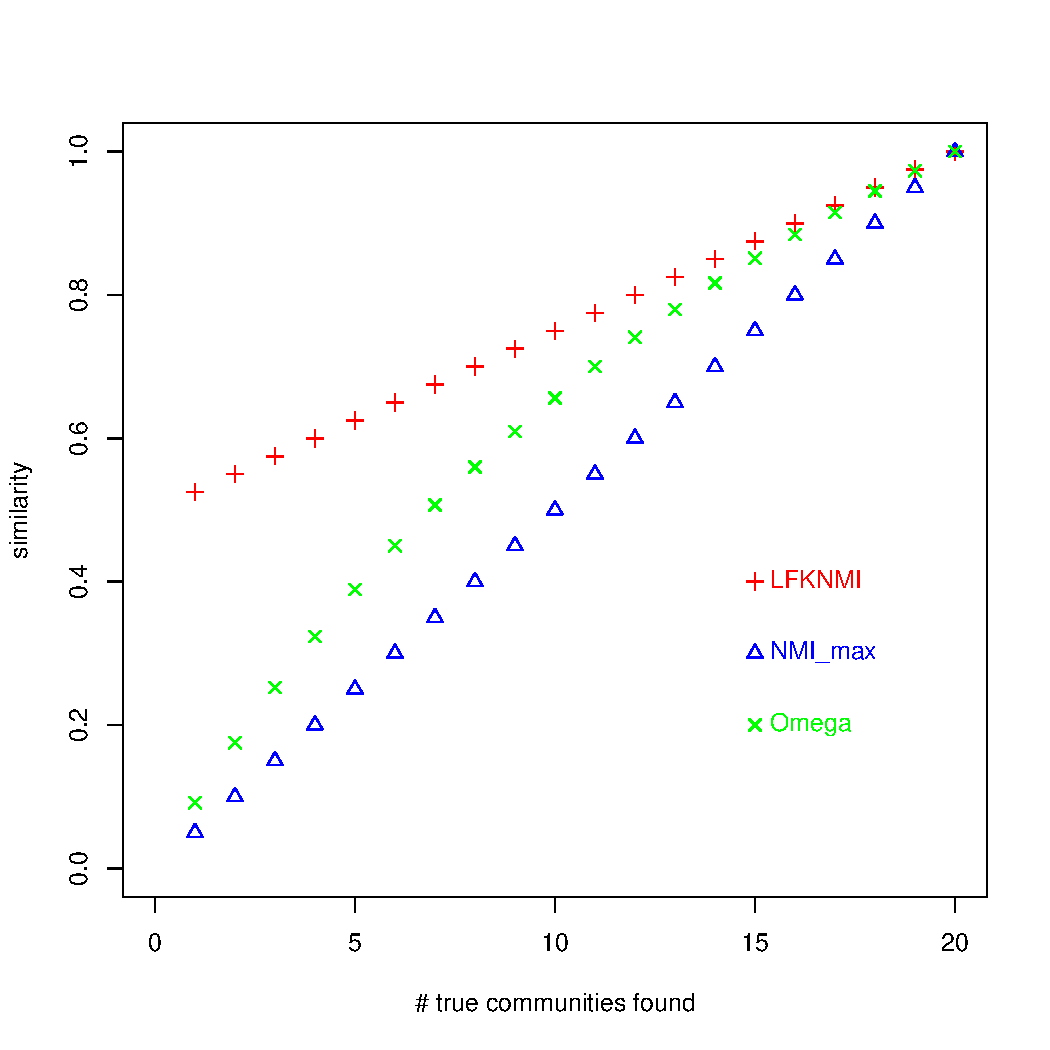
\includegraphics[width=0.5\textwidth]{plot}
\caption{As more communities are found, the score of LFKNMI and $\text{NMI}_{max}$ increase. For a small number of communities found, the intuitive result is a small value, and this is the behaviour of our proposed measure.}
\label{fig1to20}
\end{figure}

See \cref{fig1to20}. There are 200 nodes, divided into 20 communities. Each community has 10 nodes and they do not overlap.
We fix one of our covers, $X$, to be the full set of twenty communities. $Y$ contains a subset of these communities.
As we go from left to right, the number of communities in $Y$ increases from 1 to 20.

The communities in $Y$ are perfect copies of communities in $X$. Therefore, $X=Y$ when all 20 communities are used.
We see this in \cref{fig1to20} at the right, where both measures report an NMI of $1.0$.

This figure confirms the unintuitive behaviour of LFKNMI when few communities are found.
On the left of the figure, when $Y$ has only one community, the score of $0.5$ is unintuitive.

The linear relationship of our NMI$_{max}$, going from 0 to 1 as the number of communities in $Y$ increases, is intuitive.

\section{conclusion}

We have identified unintuitive behaviour in the version of NMI proposed by \lfk . We have identified the root
cause of the behaviour and shown how the use of a conventional normalization can lead to the expected behaviour.

A simple experiment was performed to confirm the existence of the unintuitive behaviour and demonstrate
the more intuitive behaviour.

There are a variety of normalized measures to measure the similarity of covers.
There is no unique set of evaluation criteria to decide on the best, but we suggest that our measure
is a more intuitive application of mutual information.







%\section{Experiments to do}
%\begin{itemize}
	%\item X versus a subset of X. (already done; as expected)
	%\item \emph{constant baseline property} independent clusterings should result in 0. Randomly rename nodes? I hypothesize LFK will be noisier.
	%\item LFM2: fullCollection versus the first grouping.
	%\item Redo the community finding algorithm plots. Will the order of the algorithms change?
%\end{itemize}

%\bibliographystyle{IEEEtran}
\bibliographystyle{unsrtnat}
%\bibliographystyle{plain}
\bibliography{community}
\end{document}
